\section{Data generation}
\label{sec:data}

\textbf{Sampling.} Each of the four transistor datasets (NMOS ON, NMOS OFF, PMOS ON, PMOS OFF) draws every input independently with a fixed seed (20261024) and a separate random stream per quantity. $V_{DD}$ is drawn first: uniform over $0.9\,\mathrm{V}\pm10\%$ ($0.81$ to $0.99$ V). The drain and source voltages $V_d$, $V_s$ are then independent uniform draws on $[0,V_{DD}]$. Width is uniform from $L_{min}$ to $8L_{min}$ (\SIrange{32}{256}{\nano\meter}) and temperature is uniform from $-40$ to \SI{125}{\celsius}. The five process parameters vth0, toxe, ndep, u0 and xj are drawn uniformly within $\pm10\%$ of the value in the model file, separately for NMOS and PMOS. For PMOS, vth0 stays negative. Gate and body voltages are fixed by the case (NMOS ON: $V_g=V_{DD}$, $V_b=0$; NMOS OFF: $V_g=V_b=0$; PMOS ON: $V_g=0$, $V_b=V_{DD}$; PMOS OFF: $V_g=V_b=V_{DD}$). Because $V_s$ varies independently, ``ON'' and ``OFF'' describe the gate bias, not a guarantee of strong inversion or cut-off at every sample.

\textbf{Dataset size.} Each CSV has the 16 required columns (vdd, temp, w, vd, vs, vg, vb, vth0, toxe, ndep, u0, xj, id, ig, is, ib). The assignment starts from 10,000 samples per case and allows more. The transistor datasets delivered with this report have 100,000 rows per case (400,000 SPICE simulations), to raise accuracy, which the assignment allows. An earlier 10,000-row run is superseded and is not included. The gate and circuit corners are new draws.

\textbf{Split.} Each 100,000-row dataset is split at random, with the fixed seed, into 70,000 training, 15,000 validation and 15,000 test rows (70/15/15). The test rows were not used until the four final models were frozen.

\textbf{Netlists.} Every netlist (transistor, gate, circuit) contains \texttt{.options gmin=1e-18 abstol=1e-18 reltol=1e-6 vntol=1e-9}. In the single-transistor netlists each of the four terminals has its own voltage source, so the four terminal currents are measured separately (as the negative of each source current). Gate netlists are complete transistor-level cells: NAND2 and NOR2 with their internal node, and AND2 and OR2 as a NAND2 or NOR2 followed by an inverter in one netlist (not as summed separate simulations). Gate inputs are exactly 0 or $V_{DD}$. Per-corner process values replace only the five assigned parameters of the \texttt{nmos} and \texttt{pmos} model cards. The circuit netlist is one connected 112-transistor deck. Example netlists are in \texttt{netlists/}. Diffusion areas and perimeters keep the model and simulator defaults. Every gate and circuit output was checked against the logic level (below $0.2V_{DD}$ for logic 0 and above $0.8V_{DD}$ for logic 1).

\textbf{Kirchhoff check.} For every row, $|I_d+I_g+I_s+I_b|$ was compared with the sum of the absolute currents (Table~\ref{tab:kcl}). The residuals are at the numerical floor of the simulator. The larger values in the PMOS OFF case occur where the largest current is a body current of about \SI{1e-14}{\ampere}, so a residual of \SI{1e-15}{\ampere} is a large fraction of the total but is negligible in absolute terms. The rows were retained, not corrected or projected out. Spread-out rows were also compared with independently instantiated fresh model cards, to verify that the batched parameter updates are correct. The worst normalised residual is 0.014\%.

\textbf{TOXE and DTOX.} Varying TOXE alone while keeping the supplied TOXP and DTOX can trigger the BSIM warning that DTOX is ignored. TOXE remains active, as confirmed by a direct sensitivity experiment. The model file is unchanged, and TOXP, TOXM, TOXREF and the other unassigned parameters are never co-varied silently.

\begin{table}[H]
\centering\small
\caption{Kirchhoff check on the 100,000-row datasets. The threshold is $10^{-18}\,\mathrm{A}+10^{-6}\sum|I|$.}
\label{tab:kcl}
\begin{tabular}{lrrr}
\toprule
Case & Max $|\sum I|$ (A) & Max $|\sum I|/\sum|I|$ & Rows above threshold \\
\midrule
NMOS ON & $1.15\times10^{-15}$ & $9.6\times10^{-5}$ & 225 \\
NMOS OFF & $3.35\times10^{-22}$ & $7.5\times10^{-15}$ & 0 \\
PMOS ON & $3.80\times10^{-17}$ & $3.8\times10^{-6}$ & 1 \\
PMOS OFF & $8.11\times10^{-15}$ & $1.4\times10^{-4}$ & 4153 \\
\bottomrule
\end{tabular}
\end{table}

\textbf{Trend plots.} Figure~\ref{fig:trends} shows controlled SPICE sweeps (41 points per polarity and sweep), each varying one parameter around $V_{DD}=\SI{0.9}{\volt}$, $T=\SI{27}{\celsius}$ and nominal process values. OFF current rises with temperature (by a factor of 16.0 for NMOS and 11.1 for PMOS between $-40$ and \SI{125}{\celsius}). It falls as the threshold magnitude increases (NMOS vth0 from 0.320 to \SI{0.391}{\volt}: factor 0.25; PMOS vth0 from $-0.265$ to \SI{-0.217}{\volt}, i.e.\ decreasing $|$vth0$|$: factor 3.1). The ON gate current falls with oxide thickness (toxe from 0.675 to \SI{0.825}{\nano\meter} for NMOS: factor 0.079). These are the expected physical trends. The scatter plot of the random dataset (Figure~\ref{fig:scatter}) shows the same temperature and oxide trends, but a weak vth0 trend (binned-median ratio 0.74 and 0.76), because all other parameters vary at the same time. The controlled sweeps are therefore the evidence for the vth0 trend.

\begin{figure}[H]
\centering
\begin{subfigure}[t]{0.32\linewidth}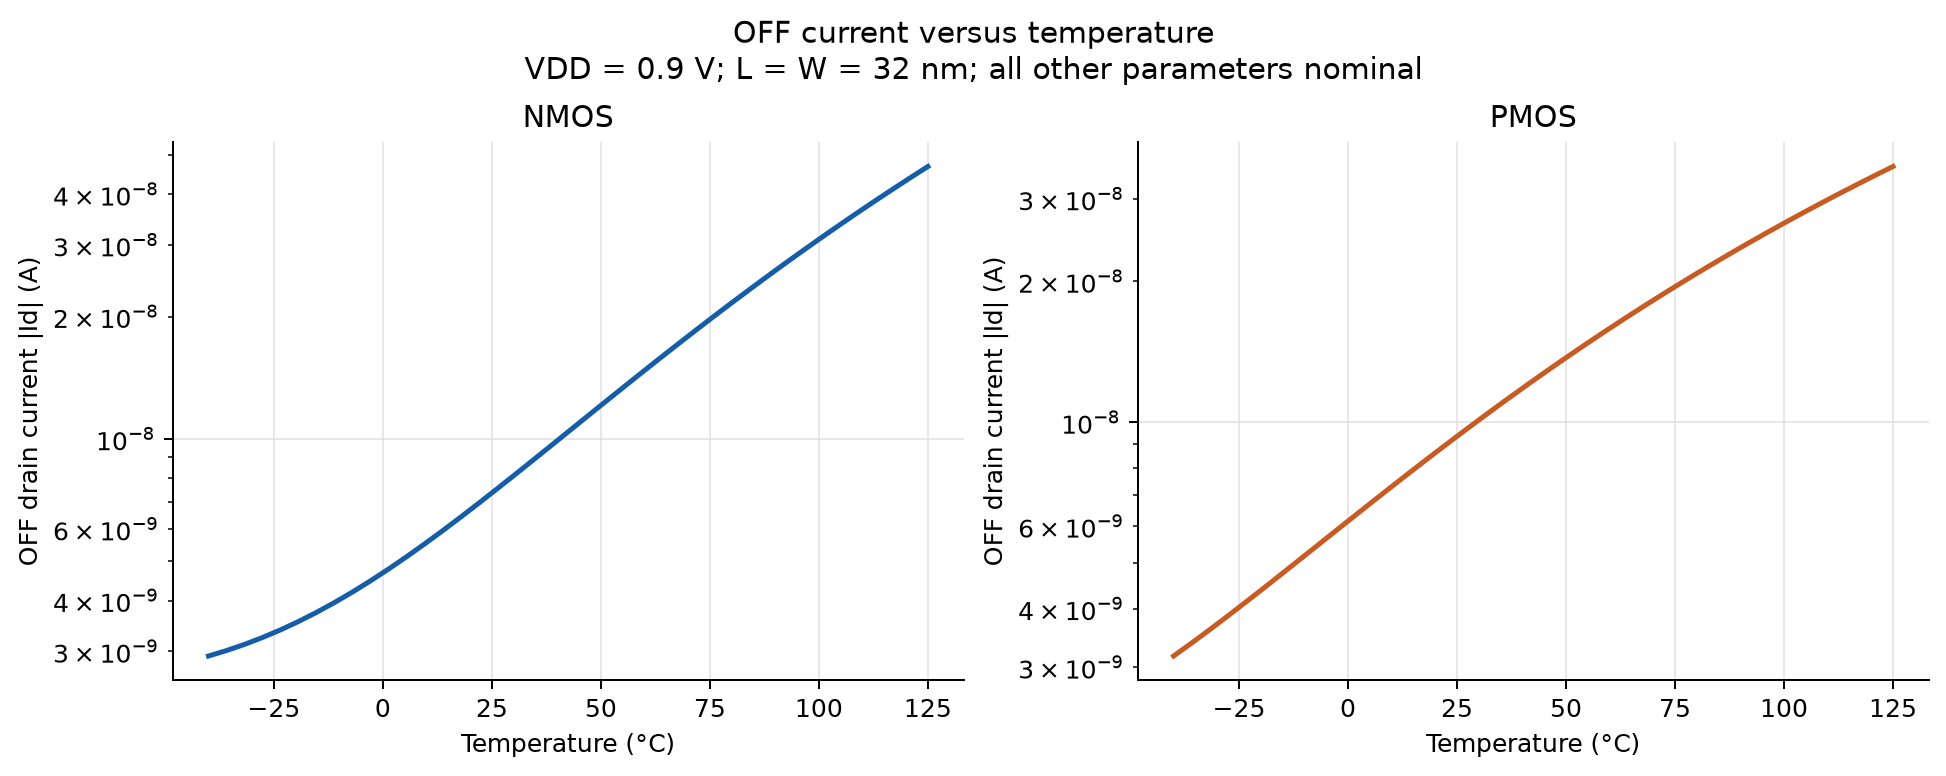
\includegraphics[width=\linewidth]{data_checks/plots/off_current_vs_temperature.png}\caption{OFF $I_d$ vs $T$}\end{subfigure}
\begin{subfigure}[t]{0.32\linewidth}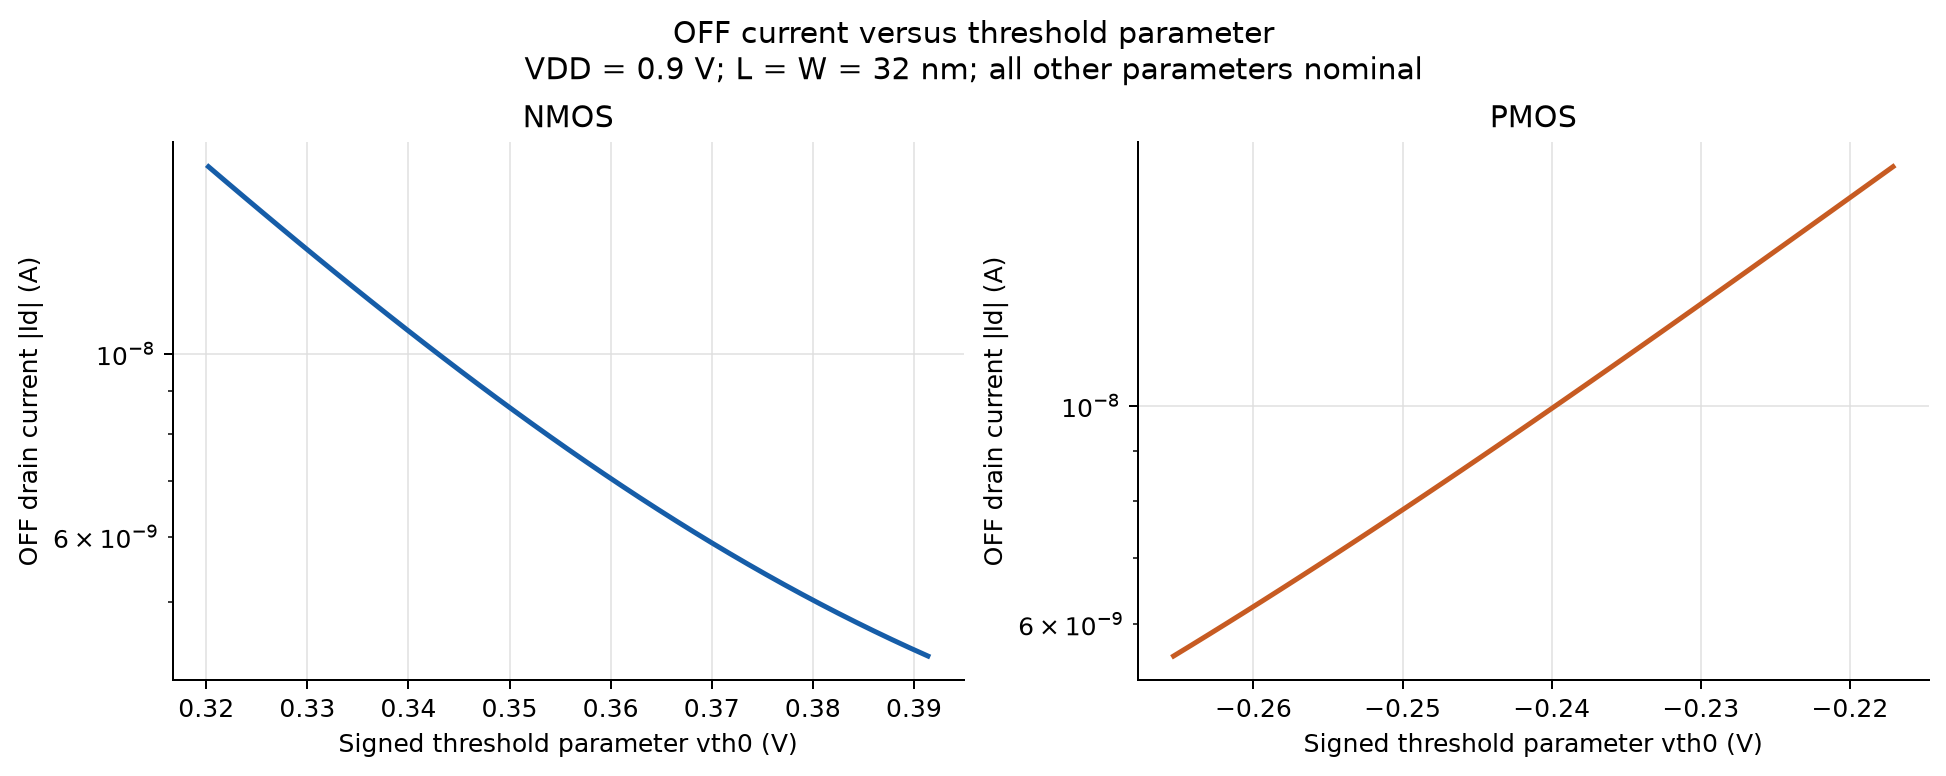
\includegraphics[width=\linewidth]{data_checks/plots/off_current_vs_vth0.png}\caption{OFF $I_d$ vs vth0}\end{subfigure}
\begin{subfigure}[t]{0.32\linewidth}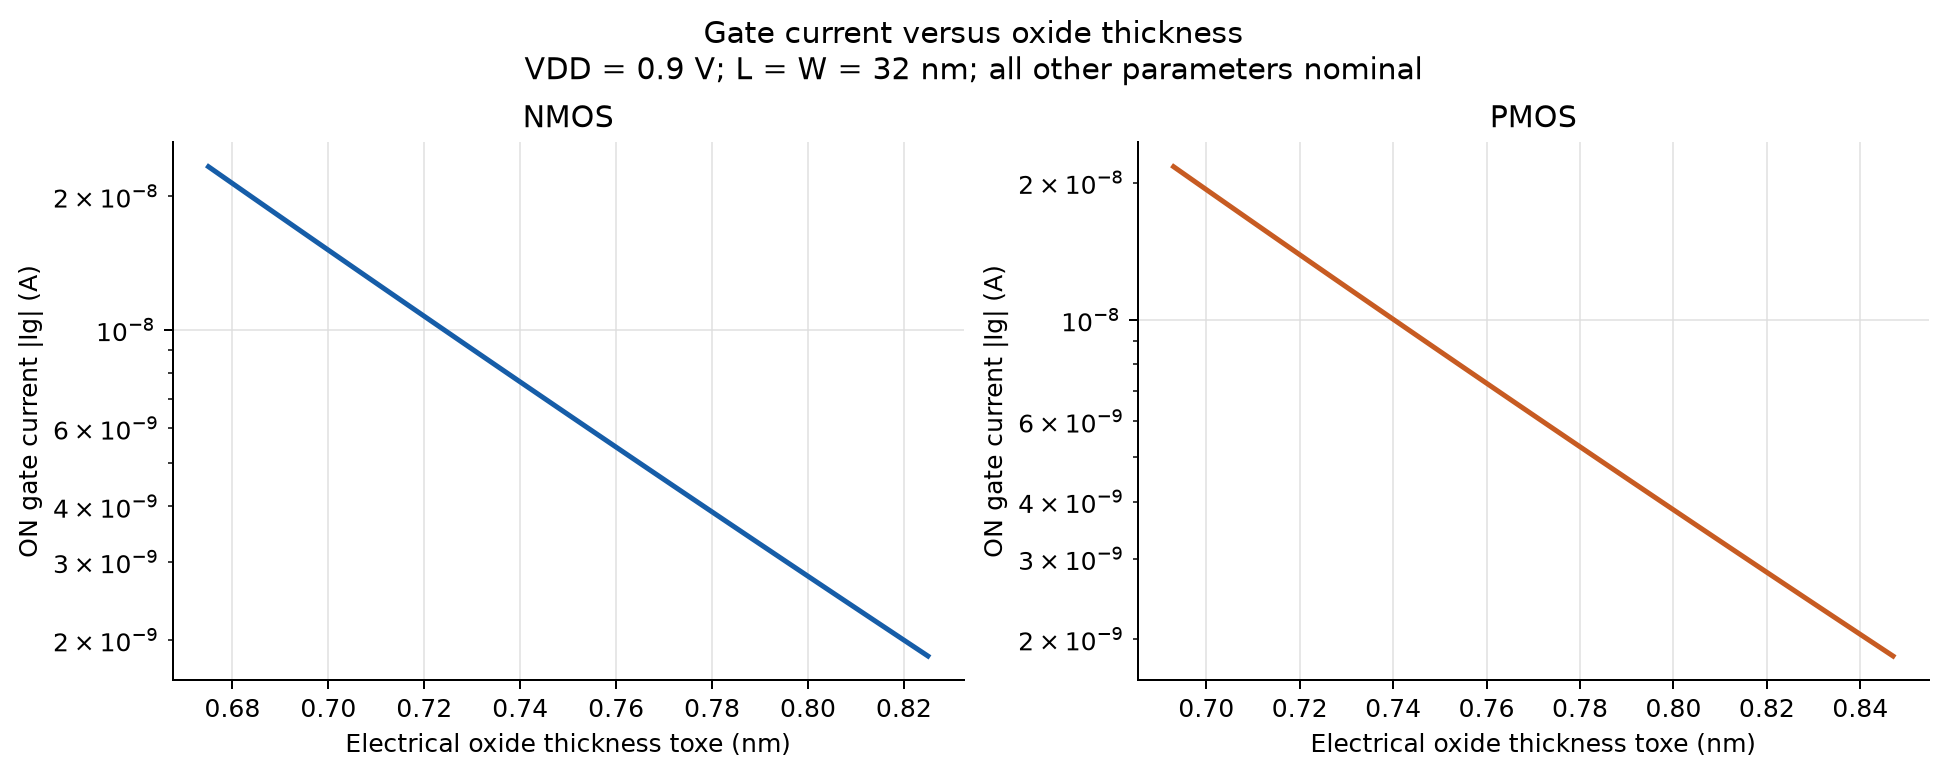
\includegraphics[width=\linewidth]{data_checks/plots/gate_current_vs_toxe.png}\caption{ON $I_g$ vs toxe}\end{subfigure}
\caption{Controlled SPICE trend sweeps.}
\label{fig:trends}
\end{figure}

\begin{figure}[H]
\centering
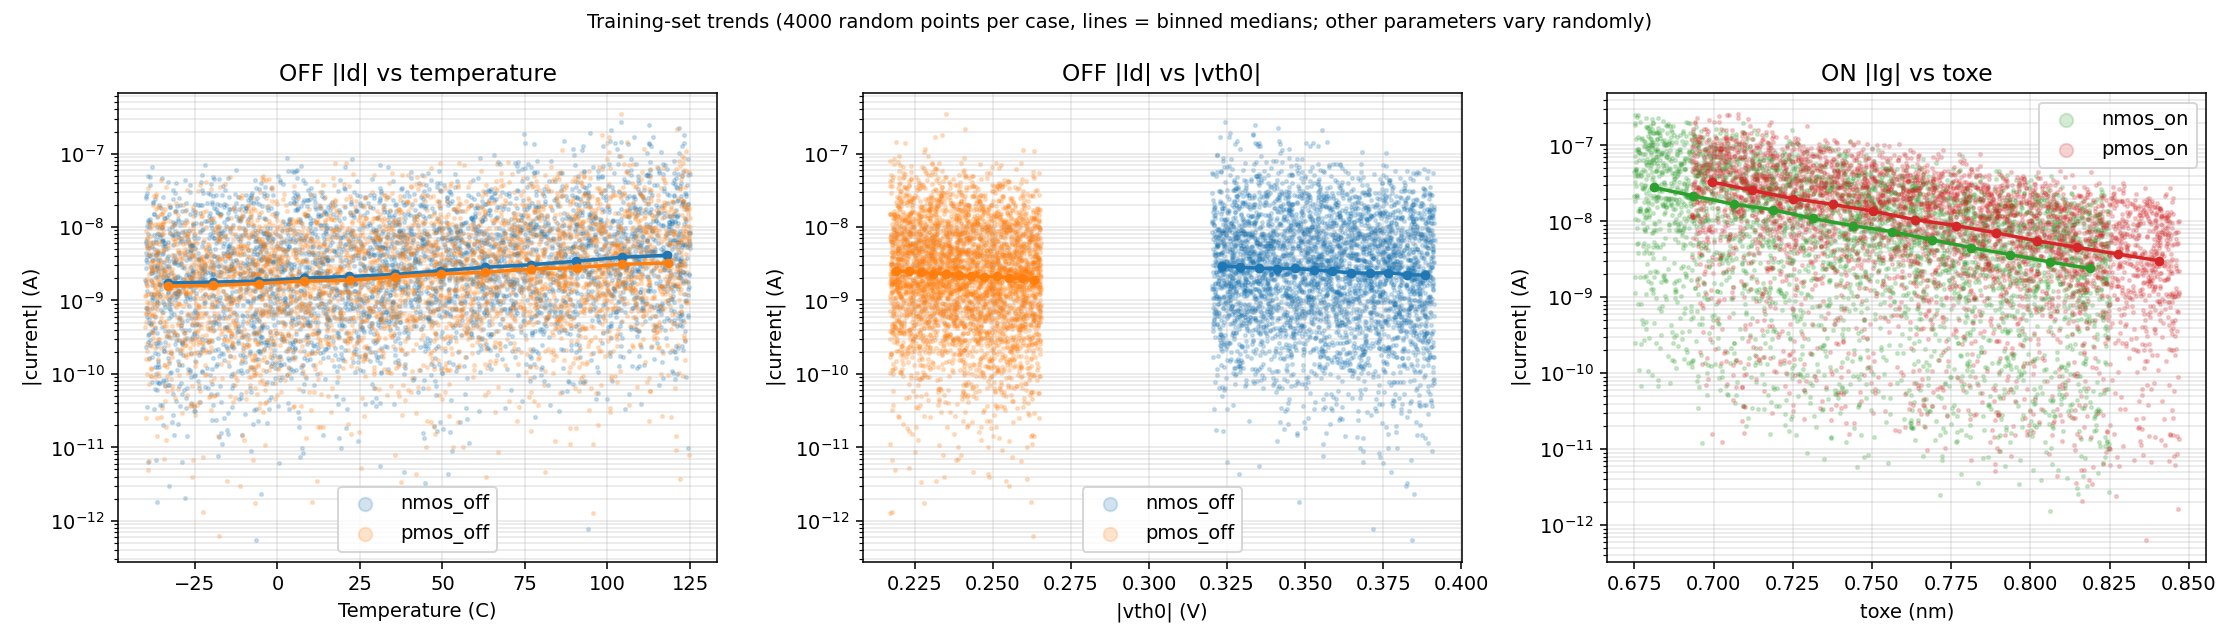
\includegraphics[width=\linewidth]{figures/analysis/trends_dataset.png}
\caption{The same quantities on the random 100,000-row datasets (binned medians). Median ratios last/first bin: OFF $|I_d|$ vs $T$ 2.4 (NMOS) and 2.1 (PMOS); ON $|I_g|$ vs toxe 0.086 (NMOS) and 0.092 (PMOS).}
\label{fig:scatter}
\end{figure}
